\documentclass[crop,tikz]{standalone}
\begin{document}
    \definecolor{trimer}{HTML}{1f77b4}

    % \begin{tikzpicture}
    %     \draw[color=blue] (0, 0) -- (4, 0) -- (4, 4) -- (0, 4) -- cycle;
    %     \draw[color=black,mark=*] plot[samples at={-180,-120,...,180},variable=\x] (\x:1);
    % \end{tikzpicture}
    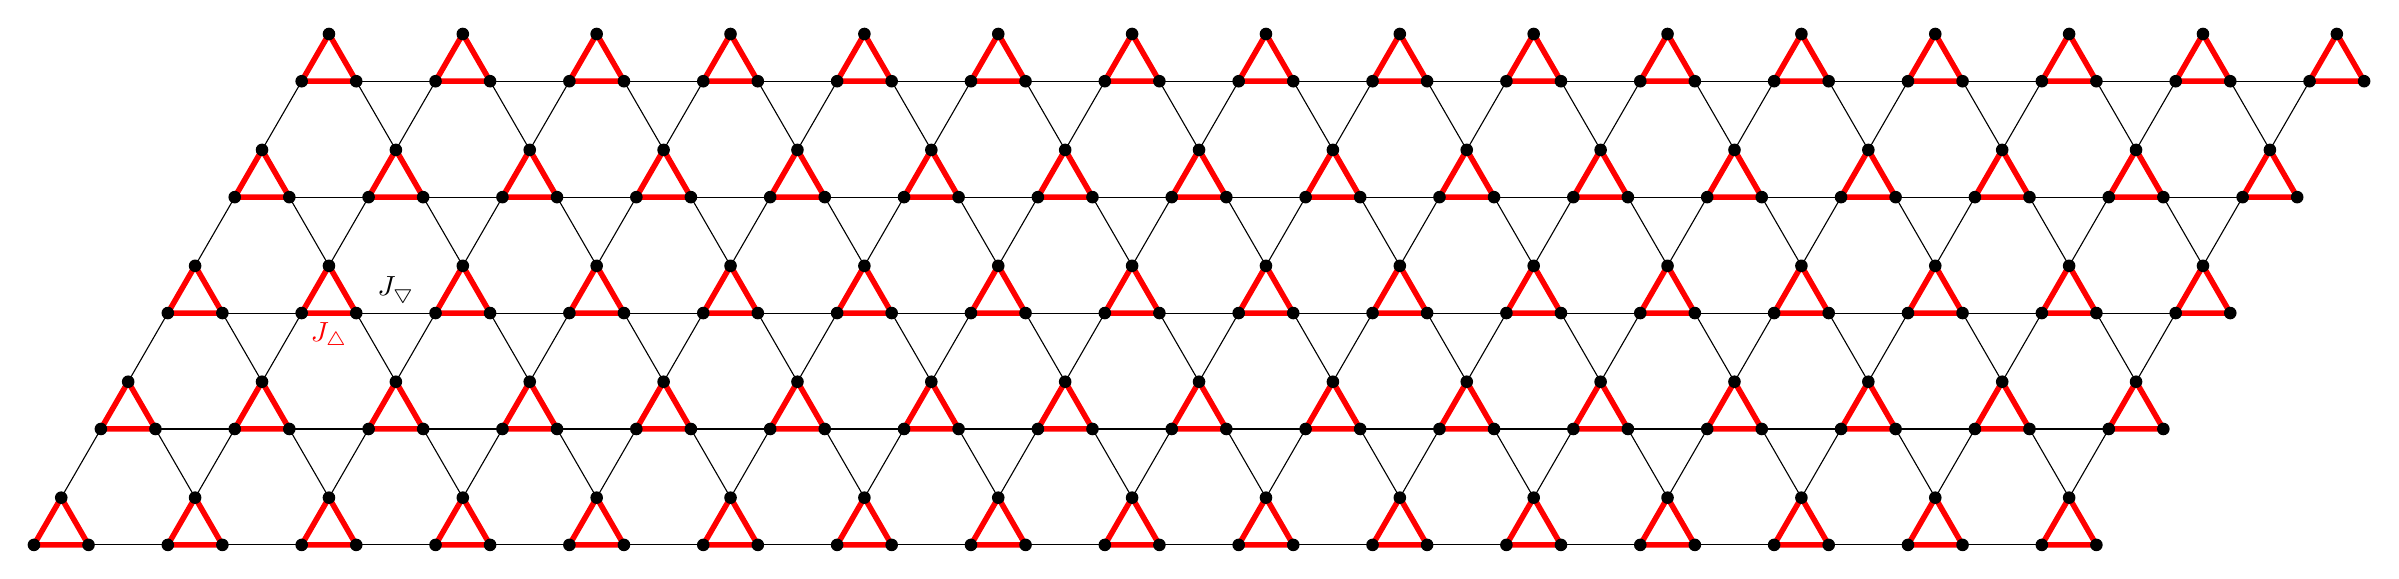
\begin{tikzpicture}[site/.style={black, font=\scriptsize}]
        \def\rad{0.4}
        \def\dx{1.7}
        \def\dy{1.7*cos(30)}
        \begin{scope}[shift={({-\dx},{-\dy})}]
            \def\Lx{15}
            \def\Ly{4}
            \def\br{1.7}

            % \clip (\br * 1.5 *0.91 -3 * \br - 0.5*\br, -\br*0.866*1.09 - \br*0.866/3) -- ++(\br * 1.98, 0) -- ++(\br, 2*\br*0.866) -- ++(-\br*1.98, 0) -- cycle;

            \foreach \x in {0,...,\Lx} {
                \foreach \y in {0,...,\Ly} {
                    \begin{scope}[shift={(\br*\x+\br*0.5*\y-3*\br, \br*0.866*\y-\br*0.866*2)}]
                        \foreach \a in {0,1,2} {\coordinate (A\x\y\a) at (120*\a-30:\rad);}
                        \draw[line width=2, red] (A\x\y0) -- (A\x\y1) -- (A\x\y2) -- cycle;
                        \foreach \a in {0,1,2} {\draw[fill=black,draw=none] (A\x\y\a) circle (0.08);}
                    \end{scope}

                    \ifnum \x > 0
                    \pgfmathtruncatemacro\xm{\x-1}
                    \draw (A\x\y2) --(A\xm\y0);
                    \ifnum \y > 0
                    \pgfmathtruncatemacro\ym{\y-1}
                    \draw (A\xm\y0) --(A\x\ym1);
                    \fi

                    \fi
                    \ifnum \y > 0
                    \pgfmathtruncatemacro\ym{\y-1}
                    \draw (A\x\y2) --(A\x\ym1);
                    \fi
                }
            }
            \draw[red,draw=none] (A122)-- node[below]{$J_\bigtriangleup$} (A120);
            \draw[draw=none] (A120) -- node[above] {$J_\bigtriangledown$} (A222);
        \end{scope}
    \end{tikzpicture}
\end{document}